% =====================================================================
%  Project Proposal -- Emergency Resource Allocation
%  HOW TO USE:
%   1. Fill in the names, course info and repo link below.
%   2. Each member compiles their OWN copy: set \MemberAtrue (Member A,
%      the experienced member who leads the repo) 
%      or \MemberAfalse (Member B). This switches the author line and the
%      Individual Learning Objectives section. Shared sections stay identical.
%   3. Name the PDF exactly as your course's naming convention requires.
% =====================================================================
\documentclass[11pt]{article}
\usepackage[margin=1in]{geometry}
\usepackage[T1]{fontenc}
\usepackage{amsmath,amssymb}
\usepackage{booktabs,tabularx,array,xltabular}
\usepackage{enumitem}
\usepackage{algorithm}
\usepackage{algpseudocode}
\usepackage{tikz}
\usetikzlibrary{positioning,arrows.meta,fit}
\usepackage[hidelinks]{hyperref}
\setlist{itemsep=2pt,topsep=4pt}

% ----------------------- EDIT THESE ---------------------------------
\newcommand{\nameA}{Firstname LastnameA}
\newcommand{\nameB}{Firstname LastnameB}
\newcommand{\course}{Course Code -- Course Name}
\newcommand{\instructor}{Instructor Name}
\newcommand{\repo}{https://github.com/YOUR-ORG/emergency-allocation-cpp}
\newif\ifMemberA
\MemberAtrue      % <-- Member B: change to \MemberAfalse
% --------------------------------------------------------------------
\newcommand{\me}{\ifMemberA\nameA\else\nameB\fi}
\newcommand{\partner}{\ifMemberA\nameB\else\nameA\fi}

\title{\textbf{When Is Greedy Good Enough?\\[2pt]
\large A Web-Based Emergency Resource Allocation System with a C++ Engine\\
Comparing Greedy, Maximum-Flow, and Min-Cost-Flow Algorithms}}
\author{\me\ \\ \small Team: \nameA, \nameB \\ \small \course\ --- \instructor}
\date{\today}

\begin{document}
\maketitle

% =====================================================================
\section{Project Title}
\textbf{When Is Greedy Good Enough? A Web-Based Emergency Resource Allocation System with a C++ Engine Comparing Greedy, Maximum-Flow, and Min-Cost-Flow Algorithms}

% =====================================================================
\section{Problem Statement and Proposed Solution}

\paragraph{Problem.}
We study the allocation of a single homogeneous relief commodity (for
example, standardized relief kits) during an initial disaster-response window
in which replenishment is unavailable. Depot stocks, site demands, urgency
weights, and feasible delivery connections are assumed known, and the
available stock may be insufficient to meet all demand. Decision makers must
decide \emph{how much} each depot sends to each affected location, subject to
depot stock, site demand, and connection capacity. When stock is short,
maximizing the number of units delivered is not enough: allocations should
also favor the most urgent and vulnerable locations and avoid leaving some
communities with nothing. Balancing efficiency, efficacy, and equity is an
established challenge in humanitarian logistics
\cite{huang2012,gutjahr2016,mostajabdaveh2025}.

\paragraph{Research question.}
Exact optimization methods for these problems are available, including
open-source solvers, but their practical use depends on model complexity,
data requirements, implementation effort, and interpretability. Greedy rules
such as ``most urgent site first, nearest depot first'' are transparent
baselines that need little computation and are easy to explain. Our project
asks:

\begin{quote}
\emph{For a capacitated single-commodity allocation model, under what
combinations of supply scarcity, network reachability, and urgency
distribution do transparent greedy policies achieve near-optimal
urgency-weighted delivery, and when do they incur substantial losses
relative to an exact network-flow benchmark?}
\end{quote}

\noindent Our aim is to characterize the performance and equity consequences
of simple allocation policies, not to replace integrated vehicle-routing
optimization.

\paragraph{Motivating example.}
Depots A and B each hold one unit. Critical site X (demand 1, weight 10)
can be served by A or B; site Y (demand 1, weight 9) can be served only by
A. If greedy serves X first from its nearest depot A, Y becomes unreachable
and $W_{\text{greedy}} = 10$. The optimum sends B to X and A to Y, giving
$W^* = 19$, a weighted gap of $(19-10)/19 \approx 47\%$. Greedy fails when
it spends scarce capacity on flexible sites before sites with few
alternatives; our experiments measure how often and how badly this happens.

\paragraph{Hypotheses.}
These are testable expectations, not established results:
\begin{itemize}
  \item[\textbf{H1}] The urgency-weighted optimality gap of greedy
        allocation decreases as effective supply availability and the number
        of alternative feasible depot connections increase.
  \item[\textbf{H2}] Greedy performs worse when early assignments consume
        capacity needed by sites with few alternative connections. The
        scarcity level at which this effect peaks will be determined
        experimentally.
  \item[\textbf{H3}] Maximum-volume allocations can have lower
        urgency-weighted value and critical-site coverage than
        urgency-aware policies; the size of this difference depends on how
        ties among maximum-volume solutions are broken.
  \item[\textbf{H4}] Maximizing urgency-weighted delivery produces less
        equitable demand fulfillment than an equity-aware (max-min fair)
        allocation, so volume, urgency-weighted benefit, and equity must be
        reported together.
\end{itemize}

\paragraph{Users.}
Emergency-management planners, NGO logistics coordinators, and researchers or
students studying allocation policies. Planners use the web interface to
build a scenario on a map, run the algorithms, and test what-if changes (a
road closes, a depot runs low); researchers use the batch mode for
reproducible experiments. ReliefRoute is a prototype for planning and policy
comparison, not a validated operational dispatch system.

\paragraph{Proposed solution.}
A full-stack application, \emph{ReliefRoute}, whose engine and server are
written in C++. A thin browser frontend handles only display and user
input; every algorithm runs in C++ on the backend. The system:
\begin{enumerate}
  \item Loads a scenario (depots, demand sites, road network) from CSV and
        DIMACS-format files, lets the user create or edit one on an
        interactive map, or generates synthetic scenarios with controllable
        parameters.
  \item Computes depot-to-site travel times with Dijkstra's algorithm and
        derives the eligible connections from the deadline.
  \item Solves the allocation with five methods:
        \begin{itemize}
          \item[(A1)] urgency-first greedy (heuristic);
          \item[(A2)] Edmonds--Karp maximum flow (maximum volume, arbitrary
                tie-breaking);
          \item[(A3)] lexicographic flow: maximum volume first, then maximum
                urgency-weighted value among maximum-volume solutions;
          \item[(A4)] urgency-weighted min-cost flow, the exact optimum of
                the urgency-weighted objective and the main benchmark;
          \item[(A5)] max-min fair allocation (equity benchmark), with any
                remaining stock then distributed by A4.
        \end{itemize}
  \item Validates each allocation, computes volume, urgency, and equity
        metrics, and saves results to CSV for analysis.
  \item Shows the result on a map (deliveries drawn from depots to sites,
        sites colored by fill rate) and in a dashboard comparing all methods
        side by side.
  \item Supports what-if analysis: closing roads or changing supplies and
        re-running instantly.
\end{enumerate}
The same C++ core also powers a command-line interface (menu and batch
mode), so the course's console-program expectations are met as well.

\paragraph{Inputs.}
\texttt{depots.csv} (id, name, supply, lat, lon), \texttt{sites.csv} (id,
name, demand, urgency weight, lat, lon), a road graph in DIMACS \texttt{.gr}
format, and run parameters (deadline $\tau$, connection capacity, cost
factor $\alpha$, seed).

\paragraph{Outputs.}
An allocation table (depot $\rightarrow$ site $\rightarrow$ units), summary
metrics per method, a side-by-side comparison, a map view and charts in
the browser, and a results CSV per experiment.

\paragraph{Mathematical model and scope.}
Let $D$ be depots with stock $s_j$, $S$ sites with demand $d_i$ and urgency
weight $w_i>0$, $t_{ji}$ the shortest travel time, and $x_{ji}\ge 0$ the
units sent (integers). A connection $(j,i)$ is \emph{eligible} only if
$t_{ji}\le\tau$, and it has a fixed capacity $u_{ji}$:
\begin{align*}
\text{maximize}\quad & \textstyle\sum_{j,i} (w_i - \alpha\, t_{ji})\, x_{ji}\\
\text{s.t.}\quad & \textstyle\sum_i x_{ji} \le s_j,\qquad
                   \sum_j x_{ji} \le d_i,\qquad 0\le x_{ji}\le u_{ji}
                   \text{ for eligible } (j,i).
\end{align*}
Demand need not be fully met and stock need not be fully used. In the main
experiments $\alpha = 0$ (pure urgency-weighted delivery); small $\alpha > 0$
is a sensitivity analysis that discourages long trips. The model makes these
explicit simplifications:
\begin{itemize}
  \item one homogeneous commodity; supplies and response teams are not mixed;
  \item static allocation in a single period, with no replenishment;
  \item the deadline is enforced only through \emph{deadline-based
        reachability} (precomputed eligible connections); shared road
        bottlenecks, flows over time, and vehicle tours or multiple trips are
        not modeled;
  \item a road closure changes travel times and therefore which connections
        are eligible.
\end{itemize}
Under these assumptions the problem is a min-cost flow problem, so A4 is
exact. A4 uses costs $\alpha t_{ji}$ on depot--site arcs and $-w_i$ on
site--sink arcs and stops when no negative-cost augmenting path remains, which
allows unmet demand and unused stock. A3 runs the same successive-shortest-path
method until no augmenting path remains at all. A2 maximizes $\sum x_{ji}$
only. A1 is a heuristic with fully specified tie-breaking: sites by urgency
(descending), then demand (descending), then ID; depots by travel time, then
ID. A5 finds the largest common fill rate $\lambda$ such that every site with
at least one eligible connection can receive $\lfloor \lambda d_i \rfloor$
units.

\subsection*{Literature Review}
The review was split between the two members. \nameA\ covered network-flow
and allocation algorithms (Part~A); \nameB\ covered humanitarian logistics,
equity measures, and data (Part~B). The combined findings define the gap our
project addresses.

\paragraph{Part A --- Allocation and network-flow algorithms (\nameA).}
Distributing a limited supply from sources to sinks under capacity limits is
a classic network-flow problem. The Edmonds--Karp algorithm finds a maximum
flow using shortest (BFS) augmenting paths and runs in polynomial time
$O(VE^2)$ \cite{edmonds1972}; standard references present max-flow, min-cost
flow, and the successive-shortest-path method together with their complexity
\cite{ahuja1993,clrs}. Min-cost flow is the natural tool when units are not
interchangeable in value, because arc costs can encode travel time and,
with negative costs on site arcs, priority. Network-flow techniques have
been applied directly to emergency settings; for example, Dressler et al.\
use flow models to assign evacuees to building exits \cite{dressler2010}.
Greedy rules are widely used as fast, explainable baselines. In epidemic
response, Long, Nohdurft, and Spinler compared a greedy policy, a myopic
linear program, and approximate dynamic programming for placing Ebola
treatment units and found that the myopic optimization approach performed
best \cite{long2018}. Earlier work on prioritized allocation in stressed
communication networks shows the same tension: first-come-first-served or
priority-blind schemes serve important demand poorly under overload
\cite{beard2001}. Together these suggest that greedy can be adequate in some
regimes and poor in others, but the boundary between those regimes is rarely
mapped systematically for static allocation on networks.

\paragraph{Part B --- Humanitarian logistics, equity, and data (\nameB).}
Reviews of emergency-logistics optimization describe a large body of
models for facility location, stock pre-positioning, and relief
distribution, most solved with mathematical programming
\cite{caunhye2012}. A recurring theme is that cost-efficiency alone is the
wrong objective after a disaster. Huang, Smilowitz, and Balcik distinguish
efficiency, efficacy (speed and sufficiency of delivery), and equity, and
show that each objective changes the structure of good routes and
allocations \cite{huang2012}. Gralla, Goentzel, and Fine elicited expert
preferences among such objectives for aid delivery \cite{gralla2014}, and
Gutjahr and Nolz survey multicriteria optimization in humanitarian aid
\cite{gutjahr2016}. Recent work models scarcity explicitly:
Mostajabdaveh, Salman, and Gutjahr minimize a Gini-based measure of inequity
in unmet demand together with travel time, solve it with branch-and-price,
and report large inequity reductions without loss of efficiency on
earthquake data \cite{mostajabdaveh2025}. For realistic inputs, the
CDC/ATSDR Social Vulnerability Index ranks communities on census variables
for disaster planning \cite{flanagan2011}, and public federal datasets
(OpenFEMA, Census population estimates, HIFLD facilities, DIMACS road
networks \cite{dimacs2009}) allow de-identified, reproducible case studies.

\paragraph{Gap and our contribution.}
The equity-aware literature relies mainly on exact mathematical programs
whose deployment depends on model complexity, data, and implementation
effort, while simple greedy rules are attractive because they are fast and
easy to explain. We found little work that systematically measures how
far greedy and plain max-flow fall from the urgency-weighted optimum, and how
they compare on equity, \emph{as a function of} scarcity, network
reachability, and urgency distribution. Our project provides that map using
only polynomial-time algorithms implemented from scratch, validated against an
exact solver, and evaluated on both synthetic and real public data.
(We will extend this review throughout the project; the gap statement will
be re-checked before any submission for publication.)

\paragraph{Why we chose this problem.}
It combines the graph algorithms, sorting, and searching from our course with
a socially meaningful application. It is also small enough to implement fully
in one term yet open enough that a careful experimental study can produce a
genuine finding: a practical map of when a simple, explainable rule is safe to
use.

% =====================================================================
\section{Team Structure, Contributions, and Objectives}

\subsection*{Team Objectives}
\begin{itemize}
  \item Build a working full-stack application: a C++ engine and REST
        server, a browser frontend, and a C++ command-line interface, all
        sharing one algorithm core that implements five allocation methods.
  \item Decompose the program into small, reusable, individually tested
        functions.
  \item Implement our own sorting (merge sort), searching (binary search,
        BFS), and graph algorithms (Dijkstra, Edmonds--Karp, successive
        shortest paths) rather than relying on library black boxes.
  \item Read, process, and save data with CSV and DIMACS text files.
  \item Derive time and space complexity for every algorithm and confirm it
        experimentally.
  \item Run a reproducible experimental study (fixed seeds, scripted runs)
        and a real-data case study.
  \item Test with normal, boundary, and invalid inputs, and verify the
        optimal solver against brute force on small instances.
  \item Collaborate through GitHub with feature branches, pull requests,
        code review, and automated builds.
\end{itemize}

\subsection*{Team Member Contributions --- This Iteration}
\textbf{\nameA\ (Algorithms, backend, and repository lead)}
\begin{itemize}
  \item \emph{Completed:} literature review Part~A (allocation and
        network-flow algorithms); formal model above; pseudocode for
        Edmonds--Karp and min-cost flow; created the GitHub repository,
        branch protection rules, and the GitHub Actions CI workflow.
  \item \emph{Planned:} implement the residual-graph data structure,
        \texttt{edmondsKarp()}, \texttt{bellmanFord()}, and
        \texttt{minCostFlowAllocate()}; derive complexity bounds; write unit
        tests for the flow algorithms and the brute-force checker; build the
        C++ REST server and JSON API; review all of \nameB's pull requests;
        onboard \nameB\ to the Git workflow
        (branching, commits, pull requests) during the first iteration.
\end{itemize}
\textbf{\nameB\ (Data, evaluation, and frontend lead)}
\begin{itemize}
  \item \emph{Completed:} literature review Part~B (humanitarian logistics,
        equity measures, data); identified and documented open data sources;
        defined CSV formats; pseudocode for the main menu and greedy
        algorithm.
  \item \emph{Planned:} implement file loaders and savers, the synthetic
        instance generator, \texttt{mergeSortSites()},
        \texttt{binarySearchSite()}, \texttt{dijkstra()}, and
        \texttt{greedyAllocate()}; build the experiment harness and metrics;
        build the browser frontend (map view, scenario editor, comparison
        dashboard) on top of the API; write unit tests for these functions;
        review all of \nameA's pull requests.
\end{itemize}
\textbf{Shared:} edge-case testing of each other's code, interpretation of
results, and the final report. Both members write and test C++ code in every
iteration.

\subsection*{Individual Learning Objectives (\me)}
\ifMemberA
I have completed similar C++ projects before, so my objectives focus on
taking existing skills to a research-quality level:
\begin{itemize}
  \item Engineer the flow algorithms for performance (Johnson potentials,
        profiling, cache-friendly edge arrays) and measure the effect.
  \item Verify correctness rigorously with invariants and a brute-force
        oracle, beyond ordinary unit tests.
  \item Design and analyze experiments statistically (replication,
        confidence intervals, sensitivity analysis), and relate measured
        runtimes to theoretical complexity.
  \item Design a clean REST API in C++ that keeps the algorithm core
        independent of the web layer, and handle concurrent requests and
        input validation safely.
  \item Write a conference-style paper: literature positioning, methods,
        results, and limitations.
  \item Lead the repository and code-review process and mentor a teammate
        who is new to Git and GitHub.
\end{itemize}
\else
\begin{itemize}
  \item Read, validate, and write CSV and DIMACS text files robustly,
        handling malformed lines and missing files.
  \item Implement merge sort and binary search from scratch and test them on
        boundary cases.
  \item Implement Dijkstra's algorithm with a priority queue.
  \item Design a reproducible experiment harness with random seeds and
        timing, and present results as tables and plots.
  \item Validate user input in a menu-driven program.
  \item Build a frontend that calls a REST API, displays geographic data on
        a map, and charts algorithm results.
  \item Learn Git and GitHub: feature branches, clear commits, pull
        requests, resolving merge conflicts, and responding to code review.
\end{itemize}
\fi

% =====================================================================
\section{Program Design and GitHub Collaboration --- This Iteration}

\subsection{Main Features}
\begin{enumerate}
  \item Load a scenario from files, upload CSVs in the browser, or generate
        a synthetic one.
  \item Map view: depots and sites on an interactive map; click to inspect,
        add, or edit a location.
  \item Search for a site or depot by ID (binary search) and jump to it.
  \item List sites ranked by urgency (merge sort).
  \item Compute travel times from each depot over the road network
        (Dijkstra), snapping locations to the nearest road node (grid
        search).
  \item Run greedy, Edmonds--Karp, or min-cost-flow allocation and draw the
        resulting deliveries on the map.
  \item Comparison dashboard: all five methods side by side with
        metrics and charts.
  \item What-if mode: close roads or change supplies and re-run.
  \item Run batch experiments over a parameter grid (CLI or web page).
  \item Validate allocations, compute metrics, and export results as CSV.
\end{enumerate}

\subsection{Application Development}
ReliefRoute is a complete application, not only a set of algorithms. More
than 80\% of the code, and \emph{all} of the algorithmic code, is C++. The
frontend is a small HTML/CSS/JavaScript client that displays data and sends
requests; it contains no allocation, search, sort, or graph logic.

\paragraph{Architecture.}
\begin{center}
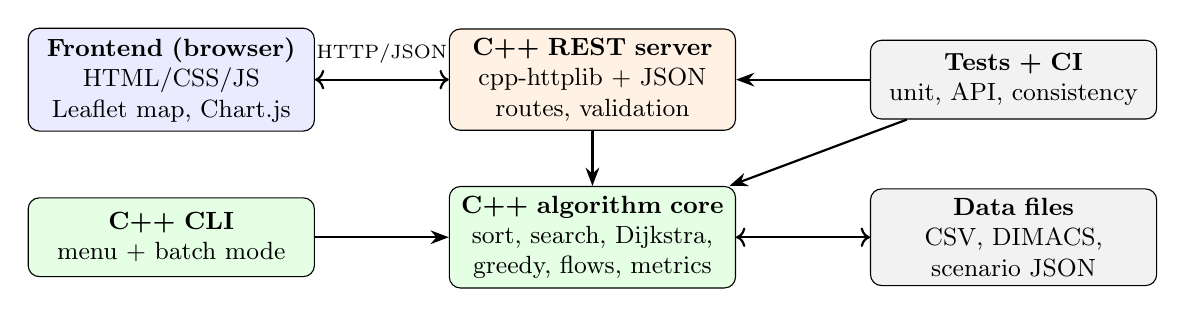
\begin{tikzpicture}[
  box/.style={draw, rounded corners, align=center, minimum height=1.0cm,
              text width=3.4cm, font=\small},
  arr/.style={-{Stealth}, thick}, node distance=0.7cm and 1.7cm]
\node[box, fill=blue!8] (fe) {\textbf{Frontend (browser)}\\HTML/CSS/JS\\Leaflet map, Chart.js};
\node[box, fill=orange!10, right=of fe] (api) {\textbf{C++ REST server}\\cpp-httplib + JSON\\routes, validation};
\node[box, fill=green!10, below=of api] (core) {\textbf{C++ algorithm core}\\sort, search, Dijkstra,\\greedy, flows, metrics};
\node[box, fill=green!10, left=of core] (cli) {\textbf{C++ CLI}\\menu + batch mode};
\node[box, fill=gray!10, right=of core] (data) {\textbf{Data files}\\CSV, DIMACS,\\scenario JSON};
\node[box, fill=gray!10, right=of api] (tests) {\textbf{Tests + CI}\\unit, API, consistency};
\draw[arr, <->] (fe) -- node[above, font=\scriptsize, yshift=2pt]{HTTP/JSON} (api);
\draw[arr] (api) -- (core);
\draw[arr] (cli) -- (core);
\draw[arr, <->] (core) -- (data);
\draw[arr] (tests) -- (api);
\draw[arr] (tests) -- (core);
\end{tikzpicture}
\end{center}
The core is a C++ library of free functions with no input/output inside the
algorithms. The REST server, the CLI, and the tests are three thin layers
over the same core, so a result in the browser is guaranteed to match the
CLI and the experiments.

\paragraph{Source layout.}
\begin{center}
\small
\begin{tabularx}{\textwidth}{@{}l l X@{}}
\toprule
\textbf{Layer / module} & \textbf{Files} & \textbf{Responsibility}\\
\midrule
Data types & \texttt{core/types.h} & Structs: \texttt{Site}, \texttt{Depot}, \texttt{Edge}, \texttt{Allocation}, \texttt{Metrics}, \texttt{Params}, \texttt{Scenario}.\\
I/O & \texttt{core/io.cpp} & Load and validate CSV, DIMACS, and scenario files; save results.\\
Generator & \texttt{core/generator.cpp} & Seeded synthetic scenarios.\\
Search/sort & \texttt{core/search\_sort.cpp} & Merge sort, binary search, grid nearest-node search.\\
Graph & \texttt{core/graph.cpp} & Road graph, Dijkstra, travel matrix, road closures.\\
Allocation & \texttt{core/greedy.cpp}, \texttt{core/flow.cpp}, \texttt{core/fair.cpp} & Methods A1--A5.\\
Evaluation & \texttt{core/metrics.cpp}, \texttt{core/experiment.cpp} & Validation, metrics, batch runs.\\
Server & \texttt{server/main.cpp}, \texttt{server/api.cpp} & HTTP routes, JSON conversion, request validation, serving the frontend files.\\
CLI & \texttt{cli/main.cpp}, \texttt{cli/menu.cpp} & Menu, batch mode, formatted console output.\\
Frontend & \texttt{web/index.html}, \texttt{web/app.js}, \texttt{web/style.css} & Map, scenario editor, dashboard; calls the API only.\\
Tests & \texttt{tests/} & Unit tests per core module; API tests; CLI-vs-API consistency.\\
\bottomrule
\end{tabularx}
\end{center}

\paragraph{REST API (backend).}
{\small
\begin{xltabular}{\textwidth}{@{}l l X@{}}
\toprule
\textbf{Method} & \textbf{Endpoint} & \textbf{Purpose (C++ function called)}\\
\midrule
\endhead
GET  & \texttt{/api/scenarios} & List saved scenarios.\\
POST & \texttt{/api/scenarios} & Upload or create a scenario (\texttt{loadSites}, \texttt{loadDepots}, validation).\\
POST & \texttt{/api/scenarios/generate} & Synthetic scenario (\texttt{generateInstance}).\\
GET  & \texttt{/api/scenarios/\{id\}/sites?sort=urgency} & Ranked sites (\texttt{mergeSortSites}).\\
GET  & \texttt{/api/scenarios/\{id\}/sites/\{siteId\}} & One site (\texttt{binarySearchSite}).\\
POST & \texttt{/api/scenarios/\{id\}/roads/close} & What-if road closure; travel matrix recomputed (\texttt{dijkstra}).\\
POST & \texttt{/api/allocate} & Run one algorithm; returns allocation and metrics.\\
POST & \texttt{/api/compare} & Run all five methods; returns a comparison.\\
POST & \texttt{/api/experiments} & Start a batch experiment; returns a job ID.\\
GET  & \texttt{/api/experiments/\{id\}} & Experiment status and results.\\
GET  & \texttt{/api/health} & Server status (used by CI).\\
\bottomrule
\end{xltabular}}
Every request body is validated in C++ before use. Malformed JSON, unknown
algorithms, negative quantities, or oversized scenarios return
\texttt{400 Bad Request} with a readable message, which the frontend shows to
the user.

\paragraph{Frontend screens.}
\begin{enumerate}
  \item \emph{Scenario map:} depots (squares sized by supply) and sites
        (circles colored by urgency); click to view or edit; search by ID;
        toggle road closures.
  \item \emph{Run panel:} choose algorithm(s) and parameters (deadline
        $\tau$, link capacity, cost factor $\alpha$); results drawn as lines
        from depots to sites, with sites shaded by fill rate.
  \item \emph{Comparison dashboard:} metrics table and bar charts (coverage,
        weighted value, gap, Jain index, runtime) for all five methods.
  \item \emph{Experiments page:} launch a parameter grid and view the
        greedy-gap heat map by scarcity and reachability.
\end{enumerate}

\paragraph{Command-line interface.}
\texttt{reliefroute-cli} offers the same operations as a text menu, and
batch mode runs experiments without prompts. \texttt{reliefroute-server}
starts the web application:
\begin{verbatim}
./reliefroute-cli --batch experiments/grid.cfg --out results/
./reliefroute-server --port 8080
\end{verbatim}

\paragraph{File formats.}
Scenarios are also saved as JSON for the web application. CSV formats:
\begin{verbatim}
sites.csv    id,name,demand,urgency,lat,lon
depots.csv   id,name,supply,lat,lon
results.csv  algorithm,seed,rho,reach,n,delivered,weighted,gap,jain,gini,ms
\end{verbatim}

\paragraph{Application roadmap.}
\begin{enumerate}[label=Iteration \arabic*:,leftmargin=*]
  \item Core data types, file I/O, search and sort, CLI menu skeleton, CI
        build. Server ``hello world'' with \texttt{/api/health}.
  \item Dijkstra, nearest-node search, greedy, Edmonds--Karp; \texttt{/api/allocate};
        frontend map that loads a scenario and draws an allocation.
  \item Min-cost flow, metrics, comparison endpoint and dashboard, scenario
        editor, what-if road closures.
  \item Generator and experiments (CLI and web page), real-data case study,
        performance tuning, README, final report.
\end{enumerate}

\subsection{Data Structures}
{\small
\begin{xltabular}{\textwidth}{@{}>{\raggedright\arraybackslash}p{0.36\textwidth} X@{}}
\toprule
\textbf{Structure} & \textbf{Purpose and justification}\\
\midrule
\endhead
\texttt{struct Site \{id, name, demand, urgency, lat, lon, node\}} &
  One record per demand location. Stored in a \texttt{vector<Site>}, sorted
  by ID so lookups can use binary search in $O(\log n)$.\\
\texttt{struct Depot \{id, name, supply, lat, lon, node\}} &
  One record per supply point, stored in a \texttt{vector<Depot>}.\\
Spatial grid: \texttt{vector<vector<int>>} buckets &
  Road nodes bucketed by latitude/longitude cell, so snapping a map location
  to its nearest road node checks only nearby cells instead of all $V_R$
  nodes.\\
\texttt{struct Scenario} + \texttt{map<string,Scenario>} &
  Holds one complete problem (sites, depots, graph, parameters, closed
  roads); the server keeps loaded scenarios by ID.\\
Road graph: \texttt{vector<vector<pair<int,int>>>} &
  Adjacency list (neighbor, travel time). Road networks are sparse
  ($E \approx 1.2V$), so this uses $O(V+E)$ memory, unlike an
  $O(V^2)$ matrix.\\
\texttt{priority\_queue} (min-heap) &
  Dijkstra frontier; gives $O((V+E)\log V)$.\\
Travel matrix \texttt{vector<vector<int>>} &
  $|D|\times|S|$ depot-to-site times, computed once and reused by all
  methods so they are compared on identical inputs.\\
\texttt{struct Edge \{to, rev, cap, cost\}} + adjacency list of edge indices &
  Residual network for flow algorithms. Storing the index of the reverse
  edge lets an augmentation update both directions in $O(1)$.\\
\texttt{queue<int>} &
  BFS for Edmonds--Karp augmenting paths.\\
\texttt{struct Allocation \{depot, site, units\}} in a vector &
  Uniform output format, so metrics and saving work for any algorithm.\\
\texttt{struct Metrics} &
  Coverage, weighted value, critical unmet demand, Jain index, Gini,
  runtime, memory.\\
\bottomrule
\end{xltabular}}

\subsection{Major Functions}
{\small
\begin{xltabular}{\textwidth}{@{}>{\raggedright\arraybackslash}p{0.38\textwidth} X@{}}
\toprule
\textbf{Function} & \textbf{Description}\\
\midrule
\endhead
\texttt{loadSites(), loadDepots()} & Read and validate CSV records; skip and report malformed lines.\\
\texttt{loadRoadGraph()} & Read a DIMACS \texttt{.gr} file into an adjacency list.\\
\texttt{generateInstance()} & Create a synthetic instance from size, scarcity $\rho$, urgency skew, reachability, and seed.\\
\texttt{saveInstance(), saveResults()} & Write instances, allocations, and metrics to CSV.\\
\texttt{showMenu(), getValidatedInt()} & Display options; read and re-prompt on invalid input.\\
\texttt{mergeSortSites()} & Stable merge sort by urgency (descending), then demand, then ID.\\
\texttt{binarySearchSite()} & Find a site by ID in the ID-sorted vector.\\
\texttt{dijkstra()} & Single-source shortest travel times from a depot node.\\
\texttt{buildTravelMatrix()} & Run Dijkstra from each depot and fill the matrix.\\
\texttt{greedyAllocate()} & Algorithm A1.\\
\texttt{buildFlowNetwork(), addEdge()} & Build the residual network with super-source and super-sink.\\
\texttt{edmondsKarp()} & A2: BFS augmenting paths; also used inside A5.\\
\texttt{bellmanFord()} & Shortest path that handles the negative arc costs.\\
\texttt{minCostFlowAllocate()} & A4 (stop at non-negative path cost) and A3 (lexicographic mode): successive shortest paths.\\
\texttt{maxMinFairAllocate()} & A5: binary search on fill rate with max-flow feasibility checks, then A4 on leftover stock.\\
\texttt{extractAllocation()} & Convert flow on depot--site arcs to \texttt{Allocation} records.\\
\texttt{validateAllocation()} & Check supply, demand, capacity, and deadline constraints.\\
\texttt{computeMetrics()} & Calculate all evaluation metrics.\\
\texttt{bruteForceOptimal()} & Exhaustive solver for tiny instances (test oracle).\\
\texttt{runExperiment()} & Loop over parameters and seeds, time each algorithm, save CSV.\\
\texttt{buildSpatialGrid(), findNearestNode()} & Bucket road nodes; find the closest node to a latitude/longitude.\\
\texttt{closeRoad()} & Remove a road edge for what-if analysis and mark travel times stale.\\
\texttt{startServer(), registerRoutes()} & Start the HTTP server and connect each endpoint to its handler.\\
\texttt{handleAllocate(), handleCompare()} & Parse and validate a request, call the core, return JSON.\\
\texttt{scenarioFromJson(), resultToJson()} & Convert between JSON and C++ structs.\\
\bottomrule
\end{xltabular}}

\subsection{Pseudocode}

\begin{algorithm}[H]
\caption{Main program flow}
\begin{algorithmic}[1]
\State $instance \gets$ empty
\Repeat
  \State \Call{showMenu}{}
  \State $c \gets$ \Call{getValidatedInt}{$0, 9$}
  \If{$c = 1$} \State $instance \gets$ \Call{loadInstanceFromFiles}{}
  \ElsIf{$c = 2$} \State $instance \gets$ \Call{generateInstance}{params}
  \ElsIf{$c = 3$} \State $k \gets$ \Call{binarySearchSite}{$instance.sites$, id}; display site $k$ or ``not found''
  \ElsIf{$c = 4$} \State $ranked \gets$ \Call{mergeSortSites}{$instance.sites$}; display $ranked$
  \ElsIf{$c \in \{5,6,7\}$}
     \State $alloc \gets$ run greedy, Edmonds--Karp, or min-cost flow
     \State \Call{validateAllocation}{$alloc$}; \Call{displayAllocation}{$alloc$}
  \ElsIf{$c = 8$} \State run all five methods; display comparison table
  \ElsIf{$c = 9$} \State \Call{runExperiment}{grid, seeds}
  \EndIf
\Until{$c = 0$}
\State \Call{saveResults}{}
\end{algorithmic}
\end{algorithm}

\begin{algorithm}[H]
\caption{Greedy allocation (A1)}
\begin{algorithmic}[1]
\Function{greedyAllocate}{$S, D, T, \tau, u$}
  \State $order \gets$ \Call{mergeSortSites}{$S$} \Comment{urgency desc, ties by demand, ID}
  \State $rem\_supply[j] \gets s_j$ for all $j$
  \For{each site $i$ in $order$}
    \State $need \gets d_i$
    \State $C \gets$ depots $j$ with $T[j][i] \le \tau$, sorted by $T[j][i]$ ascending
    \For{each $j \in C$ \textbf{while} $need > 0$}
      \State $q \gets \min(need,\ rem\_supply[j],\ u_{ji})$
      \If{$q > 0$}
        \State append $(j, i, q)$ to $alloc$
        \State $rem\_supply[j] \gets rem\_supply[j] - q$;\quad $need \gets need - q$
      \EndIf
    \EndFor
  \EndFor
  \State \Return $alloc$
\EndFunction
\end{algorithmic}
\end{algorithm}

\begin{algorithm}[H]
\caption{Edmonds--Karp maximum flow (A2; also the feasibility check inside A5)}
\begin{algorithmic}[1]
\Function{edmondsKarp}{$G, s, t$}
  \State $flow \gets 0$
  \Loop
    \State $parent \gets$ \Call{BFS}{$G, s, t$} \Comment{only edges with residual cap $> 0$}
    \If{$t$ not reached} \State \textbf{break} \EndIf
    \State $b \gets$ minimum residual capacity along the path $s \leadsto t$
    \For{each edge $e$ on the path}
      \State $e.cap \gets e.cap - b$;\quad $rev(e).cap \gets rev(e).cap + b$
    \EndFor
    \State $flow \gets flow + b$
  \EndLoop
  \State \Return $flow$
\EndFunction
\end{algorithmic}
\end{algorithm}

\begin{algorithm}[H]
\caption{Urgency-weighted min-cost flow (A4)}
\begin{algorithmic}[1]
\Function{minCostFlowAllocate}{$S, D, T, \tau, u, \alpha$}
  \State add arcs $s \to j$ (cap $s_j$, cost $0$) for each depot
  \State add arcs $j \to i$ (cap $u_{ji}$, cost $\alpha T[j][i]$) if $T[j][i] \le \tau$
  \State add arcs $i \to t$ (cap $d_i$, cost $-w_i$) for each site
  \Loop
    \State $(dist, parent) \gets$ \Call{bellmanFord}{$G, s$}
    \If{$t$ unreachable \textbf{or} $dist[t] \ge 0$} \State \textbf{break} \Comment{A3: break only if unreachable} \EndIf
    \State augment bottleneck $b$ along the path (as in Algorithm 3)
  \EndLoop
  \State \Return \Call{extractAllocation}{$G$}
\EndFunction
\end{algorithmic}
\end{algorithm}

\begin{algorithm}[H]
\caption{Max-min fair allocation (A5), using binary search}
\begin{algorithmic}[1]
\Function{maxMinFairAllocate}{$S, D, T, \tau, u$}
  \State $R \gets$ sites with at least one eligible connection \Comment{others are reported as unmet}
  \State $lo \gets 0$;\quad $hi \gets 1$
  \For{$k \gets 1$ \textbf{to} $30$} \Comment{binary search on fill rate $\lambda$}
    \State $\lambda \gets (lo + hi)/2$
    \State build network with site--sink capacity $\lfloor \lambda d_i \rfloor$ for $i \in R$
    \If{\Call{edmondsKarp}{$G$} $= \sum_{i\in R} \lfloor \lambda d_i \rfloor$}
      \State $lo \gets \lambda$ \Comment{every site can reach fill rate $\lambda$}
    \Else
      \State $hi \gets \lambda$
    \EndIf
  \EndFor
  \State $alloc_1 \gets$ allocation from the max-flow at $\lambda = lo$
  \State reduce stocks, demands, and capacities by $alloc_1$
  \State $alloc_2 \gets$ \Call{minCostFlowAllocate}{reduced instance} \Comment{use leftover stock}
  \State \Return $alloc_1 + alloc_2$
\EndFunction
\end{algorithmic}
\end{algorithm}

\begin{algorithm}[H]
\caption{Handling a web allocation request (backend)}
\begin{algorithmic}[1]
\Function{handleAllocate}{$request$}
  \State $body \gets$ parse JSON from $request$
  \If{parsing fails \textbf{or} required fields missing}
     \State \Return \texttt{400} with error message
  \EndIf
  \State $sc \gets$ scenario with ID $body.scenarioId$
  \If{$sc$ not found} \State \Return \texttt{404} \EndIf
  \If{$sc.travelStale$}
     \State $sc.T \gets$ \Call{buildTravelMatrix}{$sc$} \Comment{after road closures}
  \EndIf
  \State $start \gets$ current time
  \State $alloc \gets$ run the method named in $body.algorithm$ (A1--A5)
  \State $metrics \gets$ \Call{computeMetrics}{$alloc, sc$}; record runtime
  \State \Call{validateAllocation}{$alloc, sc$}
  \State \Return \texttt{200} with \Call{resultToJson}{$alloc, metrics$}
\EndFunction
\end{algorithmic}
\end{algorithm}

\subsection{Complexity (to be confirmed experimentally)}
Let $n=|S|$, $m=|D|$, $V$ and $E$ be the nodes and arcs of the flow network
($V = n+m+2$, $E \le n + m + nm$), $V_R, E_R$ the road graph, and $F$ the
total flow.
\begin{center}
\begin{tabular}{@{}lll@{}}
\toprule
\textbf{Algorithm} & \textbf{Time} & \textbf{Space}\\
\midrule
Merge sort & $O(n\log n)$ & $O(n)$\\
Binary search & $O(\log n)$ & $O(1)$\\
Nearest road node (grid) & $O(k)$ avg., $k$ = nodes in nearby cells & $O(V_R)$\\
Travel matrix ($m\times$ Dijkstra) & $O(m(V_R+E_R)\log V_R)$ & $O(V_R+E_R+nm)$\\
Greedy (A1) & $O(n\log n + nm\log m)$ & $O(nm)$\\
Edmonds--Karp (A2) & $O(VE^2)$ & $O(V+E)$\\
Lexicographic flow (A3) & $O(F\cdot VE)$ & $O(V+E)$\\
Min-cost flow, Bellman--Ford (A4) & $O(F\cdot VE)$ (pseudo-polynomial) & $O(V+E)$\\
Max-min fair (A5) & $O(K\cdot VE^2)$ + one A4 run, $K=30$ & $O(V+E)$\\
\bottomrule
\end{tabular}
\end{center}
If A3 and A4 are too slow on large instances, we will switch to Dijkstra with
Johnson potentials after one Bellman--Ford pass, which gives
$O(F\cdot E\log V)$.

\subsection{Experimental Design}
\begin{itemize}
  \item \textbf{Factors:} scarcity $\rho = \sum s_j / \sum d_i \in
        \{0.3, 0.5, 0.7, 0.9, 1.1\}$; reachability (fraction of depot--site
        pairs within $\tau$) $\in \{0.1, 0.25, 0.5, 1.0\}$; urgency skew
        (share of critical sites) $\in \{10\%, 30\%, 50\%\}$; size
        $n \in \{50, 200, 1000, 5000\}$.
  \item \textbf{Replication:} 30 random seeds per setting; report means with
        95\% confidence intervals.
  \item \textbf{Metrics} (fixed before running experiments): total
        delivered units; urgency-weighted value $W = \sum_i w_i x_i$;
        relative weighted gap $(W^* - W)/W^*$ against A4; fill rate
        $r_i = x_i/d_i$ per site; fraction of critical sites with
        $r_i \ge 0.5$; number of sites receiving nothing; Jain's index on fill
        rates, $J = (\sum r_i)^2/(n\sum r_i^2)$ \cite{jain1984}, over sites
        with $d_i > 0$ and defined as 1 when all $r_i = 0$; Gini index of
        unmet demand \cite{mostajabdaveh2025}; runtime and peak memory.
  \item \textbf{Case study:} counties under a recent FEMA major disaster
        declaration as sites, Census population as demand, SVI as urgency
        weight, HIFLD facilities as depots, and DIMACS/TIGER roads for travel
        times (Section~\ref{sec:data}).
\end{itemize}

\subsection{Initial Testing Plan}
{\small
\begin{xltabular}{\textwidth}{@{}c l X X@{}}
\toprule
\# & \textbf{Type} & \textbf{Test} & \textbf{Expected result}\\
\midrule
\endhead
1 & Normal & Hand-solved instance (2 depots, 3 sites) & Every method matches its hand-computed allocation.\\
2 & Normal & Supply exceeds demand, full reachability & Coverage $=1$ for every algorithm.\\
3 & Normal & Motivating example (Section 2) & A1 gives $W=10$; A4 gives $W^*=19$.\\
4 & Normal & 200 random tiny instances vs.\ \texttt{bruteForceOptimal()} & A4 objective equals brute force every time.\\
5 & Normal & Any instance & A3 volume equals A2 volume; A3 weighted value $\ge$ A2's; A4 weighted value $\ge$ every other method's.\\
6 & Boundary & Zero total supply & Empty allocation, metrics defined, no crash.\\
7 & Boundary & Site with no depot within $\tau$ & Site receives 0; reported as unmet.\\
8 & Boundary & One depot, one site & $x = \min(s, d, u)$.\\
9 & Boundary & Equal urgencies & Deterministic order by ID (stable sort).\\
10 & Boundary & Merge sort on empty, single, duplicate, reverse-sorted input & Correct, stable order.\\
11 & Boundary & Binary search for first, last, and missing ID & Correct index, or ``not found''.\\
12 & Boundary & $n = 5000$ sites & Completes; runtime logged.\\
13 & Invalid & Menu input \texttt{abc}, \texttt{-1}, \texttt{99} & Error message and re-prompt.\\
14 & Invalid & Missing file, or CSV line with missing field & Clear error; bad line skipped and counted.\\
15 & Invalid & Negative demand/supply or duplicate ID in file & Record rejected with message.\\
16 & Invariant & Any allocation from any algorithm & \texttt{validateAllocation()} passes.\\
17 & Invariant & Close one road, re-run A4 & Optimal weighted value never increases.\\
18 & Consistency & Same scenario via CLI and via \texttt{/api/compare} & Identical allocations and metrics.\\
19 & API normal & \texttt{POST /api/allocate} with a valid scenario & \texttt{200} and JSON matching the schema.\\
20 & API invalid & Malformed JSON, unknown algorithm, negative supply & \texttt{400} with a clear message; server keeps running.\\
21 & API boundary & Unknown scenario ID; very large scenario & \texttt{404}; size-limit message.\\
22 & A5 & Instance where one site has no eligible depot & That site is excluded from $\lambda$; others still get $\lfloor \lambda d_i\rfloor$.\\
23 & Frontend & Load scenario, run each algorithm, close a road & Map, table, and charts update; errors shown, not crashes.\\
\bottomrule
\end{xltabular}}


\subsection{Open Data Sources}\label{sec:data}
All data are public and aggregated at facility or county level. No personal
records are used.
\begin{itemize}
  \item \textbf{OpenFEMA Disaster Declarations Summaries (v2)} ---
        every federally declared disaster since 1953, one row per designated
        county; free REST API, CSV export, no key needed. \emph{Use:} choose
        affected counties (sites).
  \item \textbf{U.S. Census Bureau county population estimates
        (CO-EST2025-alldata)} --- annual county populations, 2020--2025.
        \emph{Use:} scale demand.
  \item \textbf{CDC/ATSDR Social Vulnerability Index (SVI)} --- county and
        tract percentile rankings from 16 census variables, designed for
        disaster planning \cite{flanagan2011}. \emph{Use:} urgency weights.
  \item \textbf{HIFLD Open} (hospitals, fire/EMS stations, Red Cross
        facilities, shelters) --- archived copies on DataLumos/ICPSR (e.g.\
        hospitals, doi:10.3886/E239108V1). \emph{Use:} depot locations.
  \item \textbf{9th DIMACS Implementation Challenge road networks
        (TIGER/Line)} --- road graphs for all 50 states in a plain-text
        \texttt{.gr} format that is easy to parse in C++ \cite{dimacs2009}.
        \emph{Use:} travel times via Dijkstra.
  \item \textbf{Synthetic generator (ours)} --- random geometric graphs with
        controlled $\rho$, reachability, and urgency skew; the main source
        for the experimental study.
\end{itemize}
Python is used only for one-time preprocessing (joining CSVs on county FIPS
codes). All algorithms run in C++.

\subsection{GitHub Setup}
\begin{itemize}
  \item \textbf{Repository:} \url{\repo}, private during development;
        \nameA\ created and administers it, \nameB\ has write access, and
        the instructor is added as a collaborator.
  \item \textbf{Branching:} \texttt{main} is always compiling and passing
        tests (protected, no direct pushes); \texttt{dev} is the integration
        branch; one \texttt{feature/<name>} branch per function group (e.g.\
        \texttt{feature/greedy}, \texttt{feature/edmonds-karp}).
  \item \textbf{Commits:} small and frequent (at least several per week per
        member), with imperative messages, for example ``Add BFS augmenting path to
        edmondsKarp'' or ``Fix off-by-one in binarySearchSite''.
  \item \textbf{Pull requests and review:} every PR into \texttt{dev}
        requires approval from the other member and a passing CI build; the
        reviewer checks correctness, tests, naming, and comments.
        \texttt{dev} is merged into \texttt{main} at the end of each
        iteration.
  \item \textbf{Responsibilities:} \nameA\ owns repository settings, the
        CI workflow, the flow modules, the REST server, and their tests;
        \nameB\ owns the I/O, generator, search/sort, graph, greedy, and
        experiment modules, the frontend, and their tests; both maintain the
        README and issue tracker.
  \item \textbf{Onboarding:} because \nameB\ is new to Git, the first
        iteration starts with a short walkthrough and a practice pull request;
        \nameA\ reviews early PRs in detail and explains requested changes.
  \item \textbf{Automation:} a GitHub Actions workflow compiles with
        \texttt{g++ -std=c++17 -Wall -Wextra -O2} (via CMake), runs the unit
        tests, starts the server, and runs the API tests with \texttt{curl} on
        every push and PR.
  \item \textbf{README:} project description and research question; data
        sources and preprocessing steps; build instructions; run instructions
        for the web application, the CLI menu, and batch mode; API reference;
        screenshots; file formats; how to
        reproduce every experiment (seeds and scripts); current progress
        checklist per iteration.
\end{itemize}

% =====================================================================
\section{Tools and Programming Language}
% Member B: check your column and change any entry that is wrong.
\noindent Skill status: \textbf{A} = \nameA, \textbf{B} = \nameB.
{\small
\begin{xltabular}{\textwidth}{@{}>{\raggedright\arraybackslash}p{0.30\textwidth} X c c@{}}
\toprule
\textbf{Tool} & \textbf{Purpose} & \textbf{A} & \textbf{B}\\
\midrule
\endhead
C++17 & Primary language for all algorithms and the application & Existing & Existing\\
g++ (GCC) & Compiler; also used in CI & Existing & Existing\\
Visual Studio Code & Editor with C++ extension & Existing & Existing\\
GDB / VS Code debugger & Debugging flow and graph code & Existing & New\\
Git and GitHub & Version control, branches, PRs, reviews & Existing & New\\
GitHub Actions & Automated build and test on each push & Existing & New\\
CSV / DIMACS text files & Input and output data & Existing & New\\
Python (pandas, matplotlib) & Data preprocessing and plots only & Existing & New\\
\LaTeX & Proposal and final report & Existing & New\\
CMake & Build system for core, server, CLI, tests & Existing & New\\
cpp-httplib & Header-only C++ HTTP server library & Existing & New\\
nlohmann/json & Header-only C++ JSON library & Existing & New\\
HTML, CSS, JavaScript & Frontend user interface & Existing & New\\
Leaflet + OpenStreetMap & Interactive map in the browser & Existing & New\\
Chart.js & Charts on the comparison dashboard & Existing & New\\
curl / Postman & Testing API endpoints & Existing & New\\
\bottomrule
\end{xltabular}}

\noindent\textbf{External libraries.} The algorithm core uses only the C++
standard library (\texttt{vector}, \texttt{queue}, \texttt{priority\_queue},
\texttt{fstream}, \texttt{sstream}, \texttt{chrono}). We implement all
sorting, searching, and graph algorithms ourselves, so the complexity
analysis applies to our own code. External libraries are used only at the
edges of the system, never for algorithms:
\begin{itemize}
  \item \textbf{cpp-httplib} (header-only, MIT license): lets the C++ backend
        serve HTTP without writing a web server from scratch.
  \item \textbf{nlohmann/json} (header-only, MIT license): safe JSON parsing
        and generation for the API.
  \item \textbf{Leaflet} with OpenStreetMap tiles and \textbf{Chart.js}
        (frontend only): map display and charts.
\end{itemize}
Unit tests use our own lightweight \texttt{assert}-based helper. We will
confirm with the instructor that the web layer and these libraries are
acceptable, since the algorithms themselves remain entirely our own C++.

\medskip
\noindent For \nameA, who has completed similar projects, this project
deepens existing skills toward research quality: performance engineering,
rigorous verification, API design, experimental methodology, and
technical writing. For \nameB, it strengthens C++ function design, file
processing, and graph algorithms while introducing Git and GitHub
collaboration, automated build checks, and frontend development.

% =====================================================================
\begin{thebibliography}{99}
\bibitem{ahuja1993} R.~K. Ahuja, T.~L. Magnanti, and J.~B. Orlin.
  \emph{Network Flows: Theory, Algorithms, and Applications}.
  Prentice Hall, 1993.
\bibitem{beard2001} C.~C. Beard and V.~S. Frost.
  Prioritized resource allocation for stressed networks.
  \emph{IEEE/ACM Transactions on Networking}, 9(5):618--633, 2001.
\bibitem{caunhye2012} A.~M. Caunhye, X.~Nie, and S.~Pokharel.
  Optimization models in emergency logistics: A literature review.
  \emph{Socio-Economic Planning Sciences}, 46(1):4--13, 2012.
\bibitem{clrs} T.~H. Cormen, C.~E. Leiserson, R.~L. Rivest, and C.~Stein.
  \emph{Introduction to Algorithms}, 4th ed. MIT Press, 2022.
\bibitem{dimacs2009} C.~Demetrescu, A.~V. Goldberg, and D.~S. Johnson, eds.
  \emph{The Shortest Path Problem: Ninth DIMACS Implementation Challenge}.
  DIMACS Series in Discrete Mathematics and Theoretical Computer Science,
  vol.~74, AMS, 2009.
\bibitem{dressler2010} D.~Dressler, M.~Gro\ss, J.-P. Kappmeier, T.~Kelter,
  J.~Kulbatzki, D.~Pl\"umpe, G.~Schlechter, M.~Schmidt, M.~Skutella, and
  S.~Temme.
  On the use of network flow techniques for assigning evacuees to exits.
  \emph{Procedia Engineering}, 3:205--215, 2010.
  doi:10.1016/j.proeng.2010.07.019.
\bibitem{edmonds1972} J.~Edmonds and R.~M. Karp.
  Theoretical improvements in algorithmic efficiency for network flow problems.
  \emph{Journal of the ACM}, 19(2):248--264, 1972.
  doi:10.1145/321694.321699.
\bibitem{flanagan2011} B.~E. Flanagan, E.~W. Gregory, E.~J. Hallisey,
  J.~L. Heitgerd, and B.~Lewis.
  A social vulnerability index for disaster management.
  \emph{Journal of Homeland Security and Emergency Management}, 8(1),
  Article~3, 2011. doi:10.2202/1547-7355.1792.
\bibitem{gralla2014} E.~Gralla, J.~Goentzel, and C.~Fine.
  Assessing trade-offs among multiple objectives for humanitarian aid
  delivery using expert preferences.
  \emph{Production and Operations Management}, 23(6):978--989, 2014.
\bibitem{gutjahr2016} W.~J. Gutjahr and P.~C. Nolz.
  Multicriteria optimization in humanitarian aid.
  \emph{European Journal of Operational Research}, 252(2):351--366, 2016.
\bibitem{huang2012} M.~Huang, K.~Smilowitz, and B.~Balcik.
  Models for relief routing: Equity, efficiency and efficacy.
  \emph{Transportation Research Part E: Logistics and Transportation
  Review}, 48(1):2--18, 2012. doi:10.1016/j.tre.2011.05.004.
\bibitem{jain1984} R.~Jain, D.~M. Chiu, and W.~R. Hawe.
  A quantitative measure of fairness and discrimination for resource
  allocation in shared computer systems. Tech.\ Rep.\ DEC-TR-301, 1984.
\bibitem{long2018} E.~F. Long, E.~Nohdurft, and S.~Spinler.
  Spatial resource allocation for emerging epidemics: A comparison of
  greedy, myopic, and dynamic policies.
  \emph{Manufacturing \& Service Operations Management}, 20(2):181--198,
  2018.
\bibitem{mostajabdaveh2025} M.~Mostajabdaveh, F.~S. Salman, and W.~J. Gutjahr.
  A branch-and-price algorithm for fast and equitable last-mile relief aid
  distribution. \emph{European Journal of Operational Research},
  324(2):522--537, 2025.
\end{thebibliography}

\end{document}
